\documentclass[../main.tex]{subfiles}
\begin{document}

\section{Temperature Control of Cryostat}
We developed a Labview GUI (see Fig. \ref{fig:temp}) for the automated control of the cryostat temperature. The cryostat needs to regulate the temperature of the MKID array at $0.100 \pm 0.005$ K for stable operation of the instrument. We have confirmed operation of this software at the summit with the following specifications:
\begin{itemize}
\item 17+ continuous hours hold time at 100 mK
\item 3 hour recycle time at 4 K (MKIDs cannot be read out during this time)
\item Continuous logging of temperature and electronics rack status
\end{itemize}
Conveniently, the software allows the automated cycling of the ADR to begin at a specified time. This software runs on the Intel Nuc PC located in the MEC Electronics lack on the IR Nasmyth platform. 

The He compressor is controlled remotely and its status logged through a Labview executable provided by Cryomech. 

\begin{figure}[t]
  \centering
    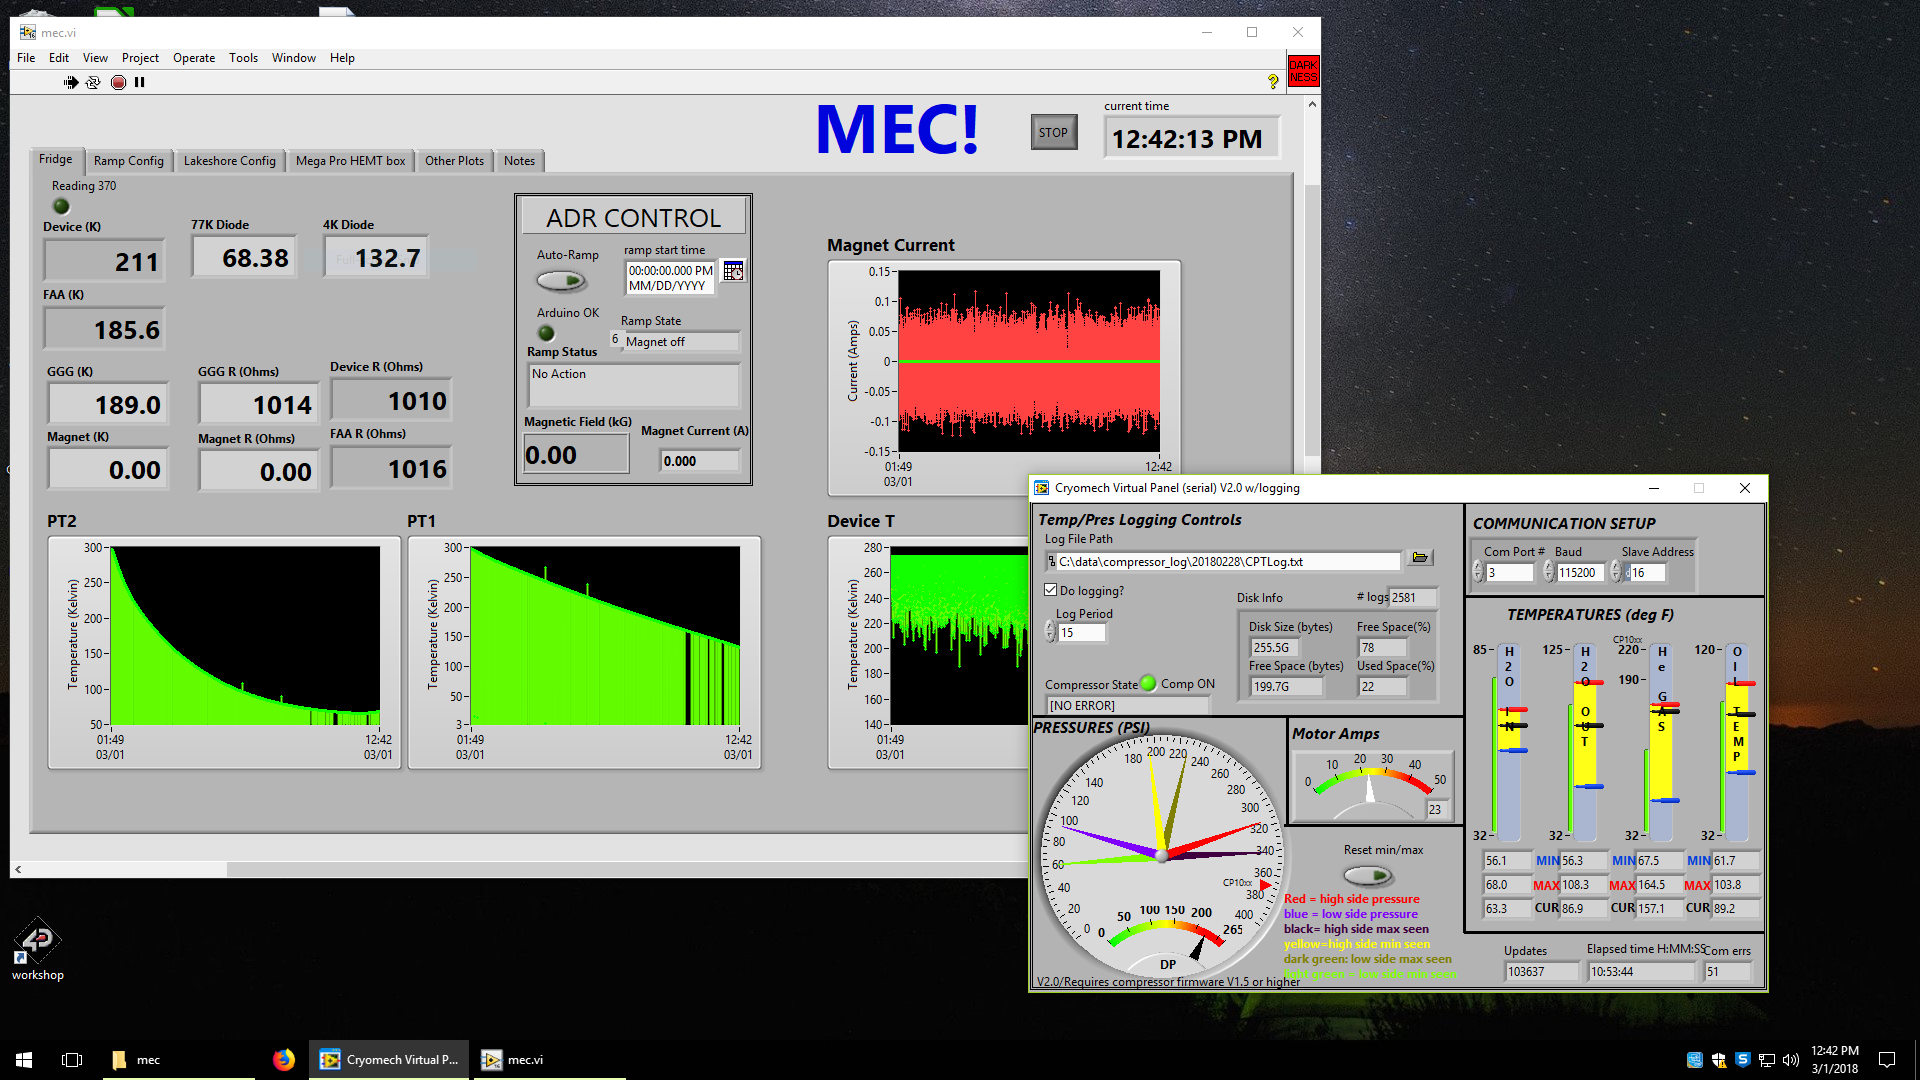
\includegraphics[width=\textwidth]{temp.png}
  \caption[MEC Temperature Control GUI]{Screenshot of MEC temperature control GUI and remote compressor control GUI.}
  \label{fig:temp}
\end{figure}

\section{Pixel Calibration and Pre-Setup}
Before operating a new MKID array every pixel must be individually calibrated. This is done by probing the MKID array using the readout electronics (see Section \ref{sec:readout_electronics}) and processing the optimal operating conditions for each pixel with automated scripts. The steps are described in the following subsections.

\subsection{Resonator Frequency Identification and Power Optimization}
While each MKID pixel has a specific design frequency, its true resonant frequency is scattered due to inhomogeneities in the superconducting film and nanoprocessing. Furthermore, when temperature cycling to room temperature and back there are often semi-global shifts in the resonator frequencies possibly due to a shift in the magnetic flux traps around the feedline or resonator circuit. This means that the MKID resonant frequency is not known a priori and must be measured by examining the transmission of a frequency sweep. 

Using the digital readout we set up a random frequency comb on the DAC and sweep the local oscillator frequency in order to measure the transmission across the entire 4-8~GHz readout band. We repeat this sweep with various levels of power attenuation to attain a power sweep. Resonators are identified in the frequency sweep as loops in the IQ plane or as sharp dips in the transmission. The power sweep data is analyzed by a deep neural net using Tensor Flow in Python to determine the optimal resonator power as described in \textcite{Dodkins_2018}. 

\subsection{Choosing the LO Frequency}
Each readout board can handle resonators within 2~GHz of bandwidth as determined by the bandwidth of the DAC and enforced by an anti-aliasing filter. We choose a local oscillator frequency in the middle of the band; around 5~GHz for the low frequency half or around 7~GHz for the high frequency half. We can not read out resonators that are more than $\pm1$~GHz away from the LO or within 250~KHz. Furthermore, we want to avoid tones in the sideband aliasing across the LO on top of a different tone in the other sideband. We use a monte carlo simulation to optimize the choice of LO to read out the largest number of pixels.

\subsection{Calculating Pixel Optimal Filters}
We use the digital readout to record the phase timestream of a resonator sampled at $1~\mu s$ while illuminating the MKID array with white light. We average photon events into a template and measure the phase noise in order to build an optimal filter that is unique for each pixel. These optimal filters are loaded into the ROACH2 firmware to improve the signal-to-noise of the on-board photon triggering. 

\subsection{Determining Pixel Location in the Array (Beammapping)}
Since the 


\section{Instrument Setup, Control, and Observing Strategy}

\subsection{Readout Board Initialization}
\subsection{High Templar: Readout Setup}
\subsection{Dashboard: Instrument Control}
\subsection{Wavelength, Flat Field, and Pointing Calibration}



\end{document}